\documentclass[10pt,a4paper]{article}

\usepackage{listings}
\usepackage{graphicx}
\usepackage{float}
\usepackage[margin=0.7in]{geometry}
\usepackage{amsmath}
\DeclareMathOperator*{\argmax}{arg\,max}
\DeclareMathOperator*{\argmin}{arg\,min}

\begin{document}

\pagenumbering{Roman}
\tableofcontents
\newpage
\pagenumbering{arabic}


\section{Software Architecture}
The solution is divided into four main components: 
\begin{itemize}
    \item The \textbf{client} - responsible for interfacing with the server or other methods of data input
    \item The \textbf{pathfinding} module - handling graph search and pathing between two points in any space
    \item The \textbf{simulation} module - handling the route selection and the actual "drone control" with the use of pathfinding
    \item The \textbf{visualisation} module - responsible for generating visualisations of the output from the simulation module
\end{itemize}

Most of the inter-module design choices explained below, are fueled by the dependency inversion principle and the rest by good general OOP practice. 
Due to the size of the solution, a lot of the simpler classes are missed out of the diagrams. 
The descriptions below will revolve mostly around the key decisions in the architecture and their benefits.

\subsection{Client module}
Figure \ref{fig:client} shows the structure of the client module classes, it contains Data classes which hold the intermediate, validated and standardised data.
These intermediate classes detach the implementation from the exact shape input data. 
Since any number of formats can map to these classes, the solution is not closely related to the input data - this is very desirable. \par

The ClientService interface is used to actually create the data in the form of Data classes from the input data given. 
In the case of AQmaps the data is given via http server and so an appropriate implementing class will need to know the base URI/location of the API where sensor/map/w3w data is stored, and have access to the Http protocol.

\par 
Any other classes which will "feed" into the rest of the system, but are constructed from input data, will be declared in this module and implement the appropriate external service interfaces.

\begin{figure}[h]
    \centering
    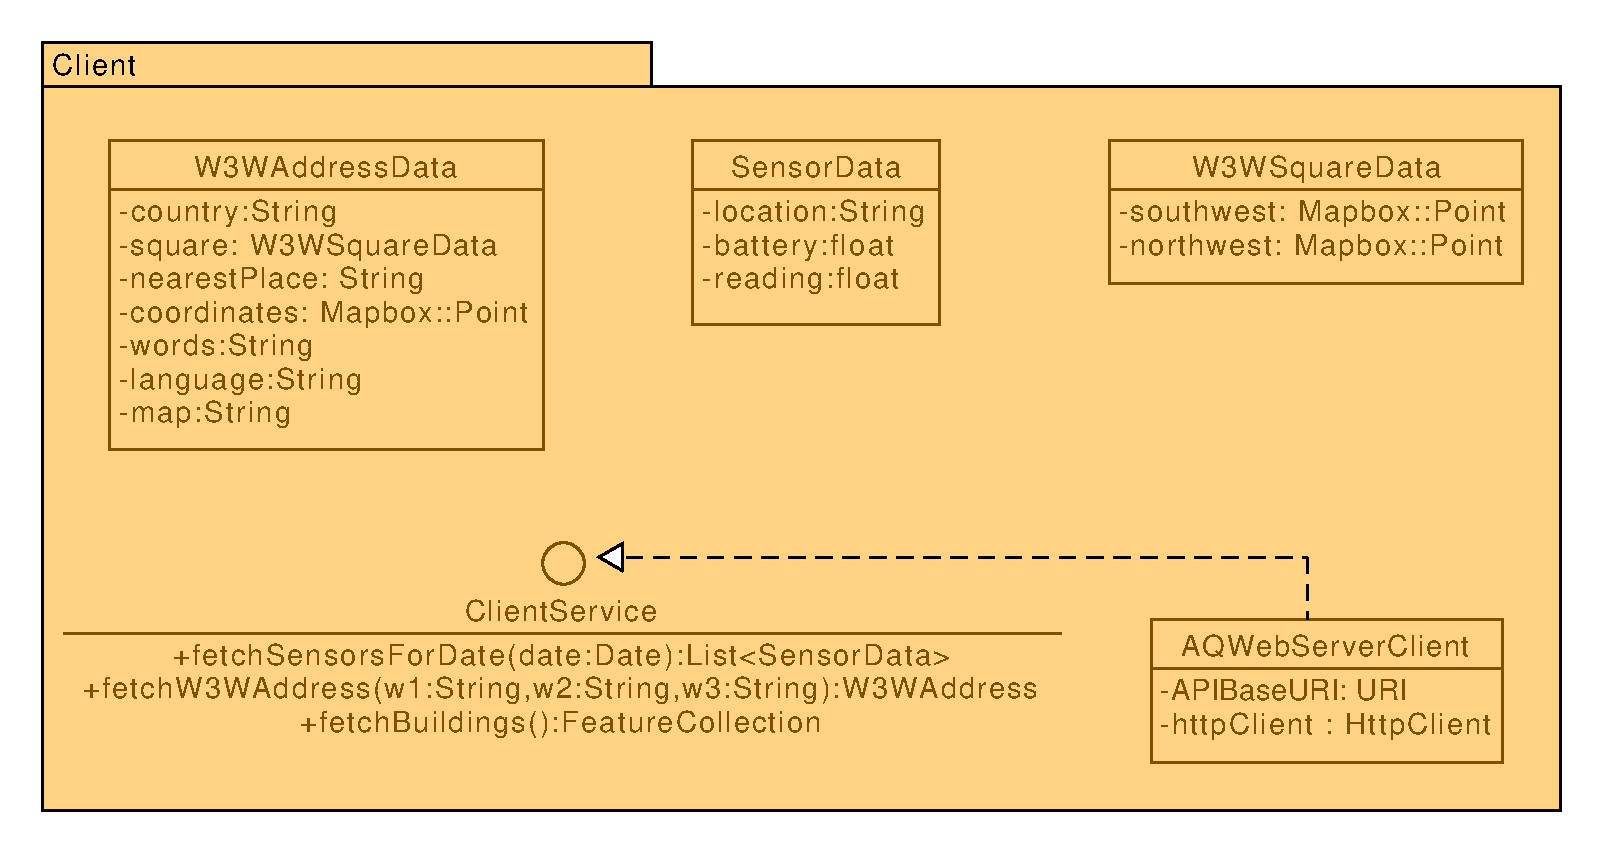
\includegraphics[width=\columnwidth]{diagrams/client.uxf.pdf}
    \caption{UML diagram of the client module}
    \label{fig:client}
\end{figure}

\subsection{Pathfinding module}
We separate the problem of pathfinding completely from the AQmap problem. This allows a broader range of techniques to be applied much more easilly.
\par 
\medskip
Figure \ref{fig:pathfinding} shows the most important classes from the pathfinding module. 
The basis of this module is formed by the SearchNode and PathfindingAlgorithm abstract classes as well as the Graph interface.
\par
The PathfindingAlgorithm class defines an abstract findPath method for finding a path to a single goal, leaving the exact way this is done to the concrete implementation. 
It is marked as abstract since we will always need to apply pathfinding to multiple goals as well, and so this class should deal with that, since this would otherwise always have to be done by the consumer.
\par
Each SearchNode is used to represent a part of the frontier of a graph search algorithm i.e. a \textbf{state} in the search space - in the pathfinding case, a path. 
These are made abstract to allow for the use of generics in such a way that each parent node is of the specific node type needed and also because nodes are expected to be annotated with problem specific data.
It is this generic parameter which propagates to the rest of the classes.
\par
Due to the fact we are mostly dealing with multiple goal pathfinding, each node should also hold a deque of goals which can be reached from it - take as an example the problem where you start at a position with 2 goals, no movement is necessary and both are reached.
\par
Pathfinding goals are represented by their own class, alternatively we could simply use coordinates as goals, 
but this would force the consumer of this functionality to always have to match the coordinates of the path returned to the goals that it needed achieved,
as opposed to simply looking through the goals achieved by each node and comparing them via reference to the deque of goals in order.

\par 
Finally the Graph interface defines the transition function from any searchNode to all its neighbours. 
PathfindingAlgorithms always accept the graph as a parameter as it forms the domain of each specific problem. 
Separating the domain from the algorithm completely makes the algorithms much more flexible and easier to unit test.

\par 
Other interfaces shown include the SpatialHash and PathfindingHeuristic, those will be used by implementing algorithms and are defined as interfaces 
to again further separate the components of algorithms from the domain. This allows us to further change the behaviour and performance of algorithms,
by swapping out their components to suit (Composition over Inheritance). 





\subsection{Simulation module}
The simulation module is responsible for: planning the route (using TSP solvers), applying pathfinding to find the detailed path required for collection, and setting the read status in sensors. 
The name stems from the fact that our sensor data collection is only simulated. This module directly interfaces with the pathfinding module as expected. 
Principles of dependency inverersion were applied to reduce coupling and increase flexibility.
\par 
\medskip
Figure \ref{fig:simulation} shows the most important classes of the simulation module. The biggest architectural choice here is the splitting of the drone into components. 
\\
This means that we keep the specific pathfinding and route planning behaviour separate from the behaviour of the drone/data collector itself.
Since it is not the job of the path or route planner to "read" any sensors, this will be the task of the drone in addition to perhaps applying some strategy
to the produced path in case it is not satysfying enough (maybe re-routing from a point with a different collection order).
\par
Another big choice is the fact that this module does not know anything about the input data, it simply defines a contract for the sensor class, letting the consumers of this module deal with 
data conversion.

\par 
The path planner component itself is further composed of the PathfindingAlgorithm and DistanceMatrix which means it only concerns itself with the 
task of translating a path of individual points it receives from the PathfindingAlgorithm to a path composed of path segments enforcing the move pattern of the drone.
\par
The PathSegment class is necessary since it is a major requirement that the collector must move in a specific pattern, this class can be used to enforce such a contract.
\par 
On the other hand CollectionOrderPlanners are only defined by their implementation and the choice of DistanceMatrix as well as the set of route optimisers. 
This choice decouples the major TSP solving strategy from the distance measure that it uses. 
\par
Both the PathPlanner and CollectionOrderPlanner interfaces have a base abstract class implementation since:
\begin{itemize}
    \item Collection order planners will always apply the set of given optimisers to the final route.
    \item They will also have to always set up the distance matrix with the given sensors 
    \item Path planners will always have to apply the given pathfinding algorithm before actually performing conversion to path segments
    \item We also use these abstract bases to enforce problem specific rules, such as the maximum number of moves, this leaves the possibility of
            straying away from those base classes if the problem changes drastically in the future.
\end{itemize}
\par 
This module also implements a specific Graph and SearchNode specific to the problem at hand. Here the ConstrainedTreeGraph produces nodes satisfying 
the angle, move length and obstacle constraints, in effect all logic to do with checking whether the collector is hitting an obstacle, or if the move length is valid etc.. is contained 
in the graph itself. This is very desirable and intentional. 
The addition of the direction field to the DirectedSearchNode further emphasizes the angle requirements, and allows for the construction of 
PathSegments from search nodes without calculating angles twice.
\par Another important class here is the abstract Sensor class. This is made abstract for two reasons:
\begin{itemize}
    \item The concrete implementation of the sensor should be done in another module, since it is more convenient for example to closely link it 
        to the input data for convenience. So according to the principle of dependency inversion we do not provide a concrete implementation in this module.
    \item The sensor cannot show any reading unless it is actually read, this can be enforced by this abstact class using the setHasBeenRead method regardless of the 
        concrete implementation/constructor.
\end{itemize}




\subsection{Visualisation module}
This module only needs to interface with the output classes of the simulation module, i.e. the PathSegment and Sensor classes but other than that, it is 
completely decoupled from the shape of the initial input data of the system. This is very desirable 
\par
Figure \ref{fig:visualisation} shows the UML diagram of the most important classes in the visualisation module.
\\
Classes implementing the SensorCollectionVisualiser interface generate geojson visualisations of sensor data collections.
These have access to both the flight path and the sensors and hence their readings. The AQMapGenerator is the problem specific example of implementation of such a visualiser.
\par
Using an interface like like this allows for the swapping out of visualisers at will whenever new requirements arise or current ones change.
\par 
The OutputFormatter class deals with writing the visualisations and flight paths to a file, these are made static as changes in output format are assumed to be very few in the future,
and should such changes be required, new methods can be added to the formatter.
\par 
The usage of the AttributeMap interface allows for a lot of flexibility in the way the AQMapGenerator assigns colors and symbols, and should this behaviour need to be changed, it'd be very easy to do.
\begin{figure}[H]
    \centering
    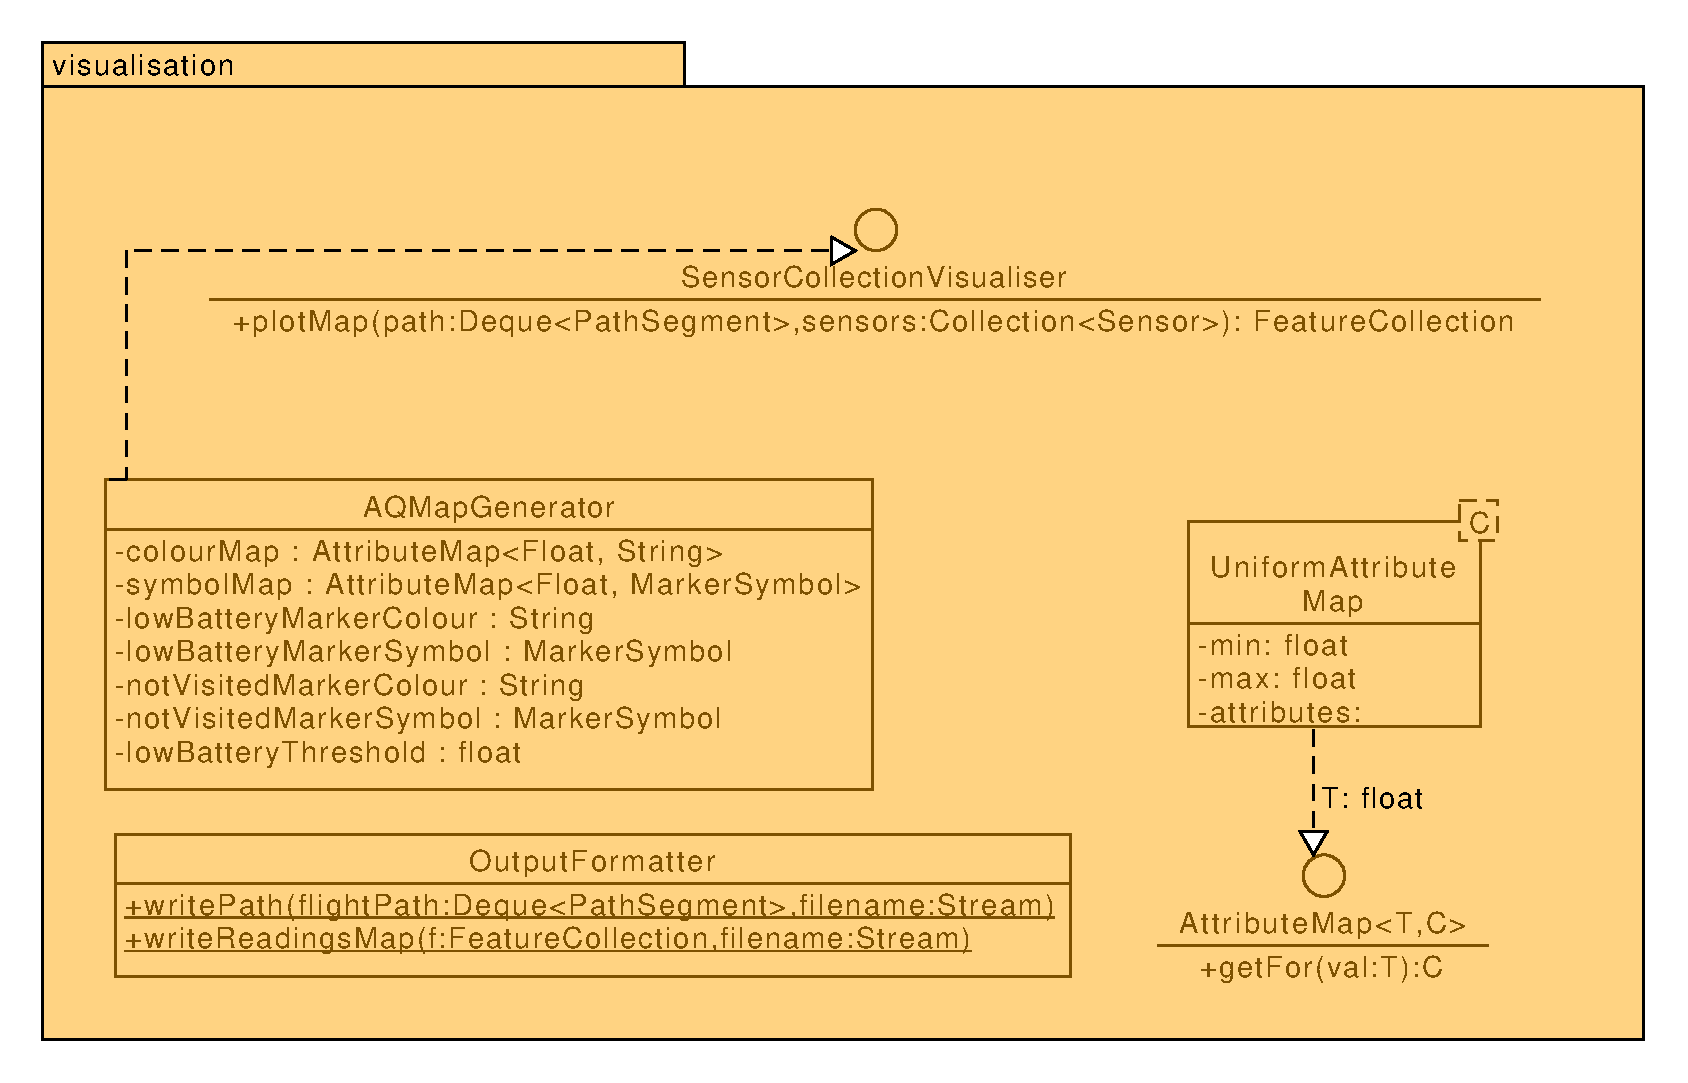
\includegraphics[width=\columnwidth]{diagrams/visualisation.uxf.pdf}
    \caption{UML diagram of the Visualisation module}
    \label{fig:visualisation}
\end{figure}
\begin{figure}[H]
    \centering
    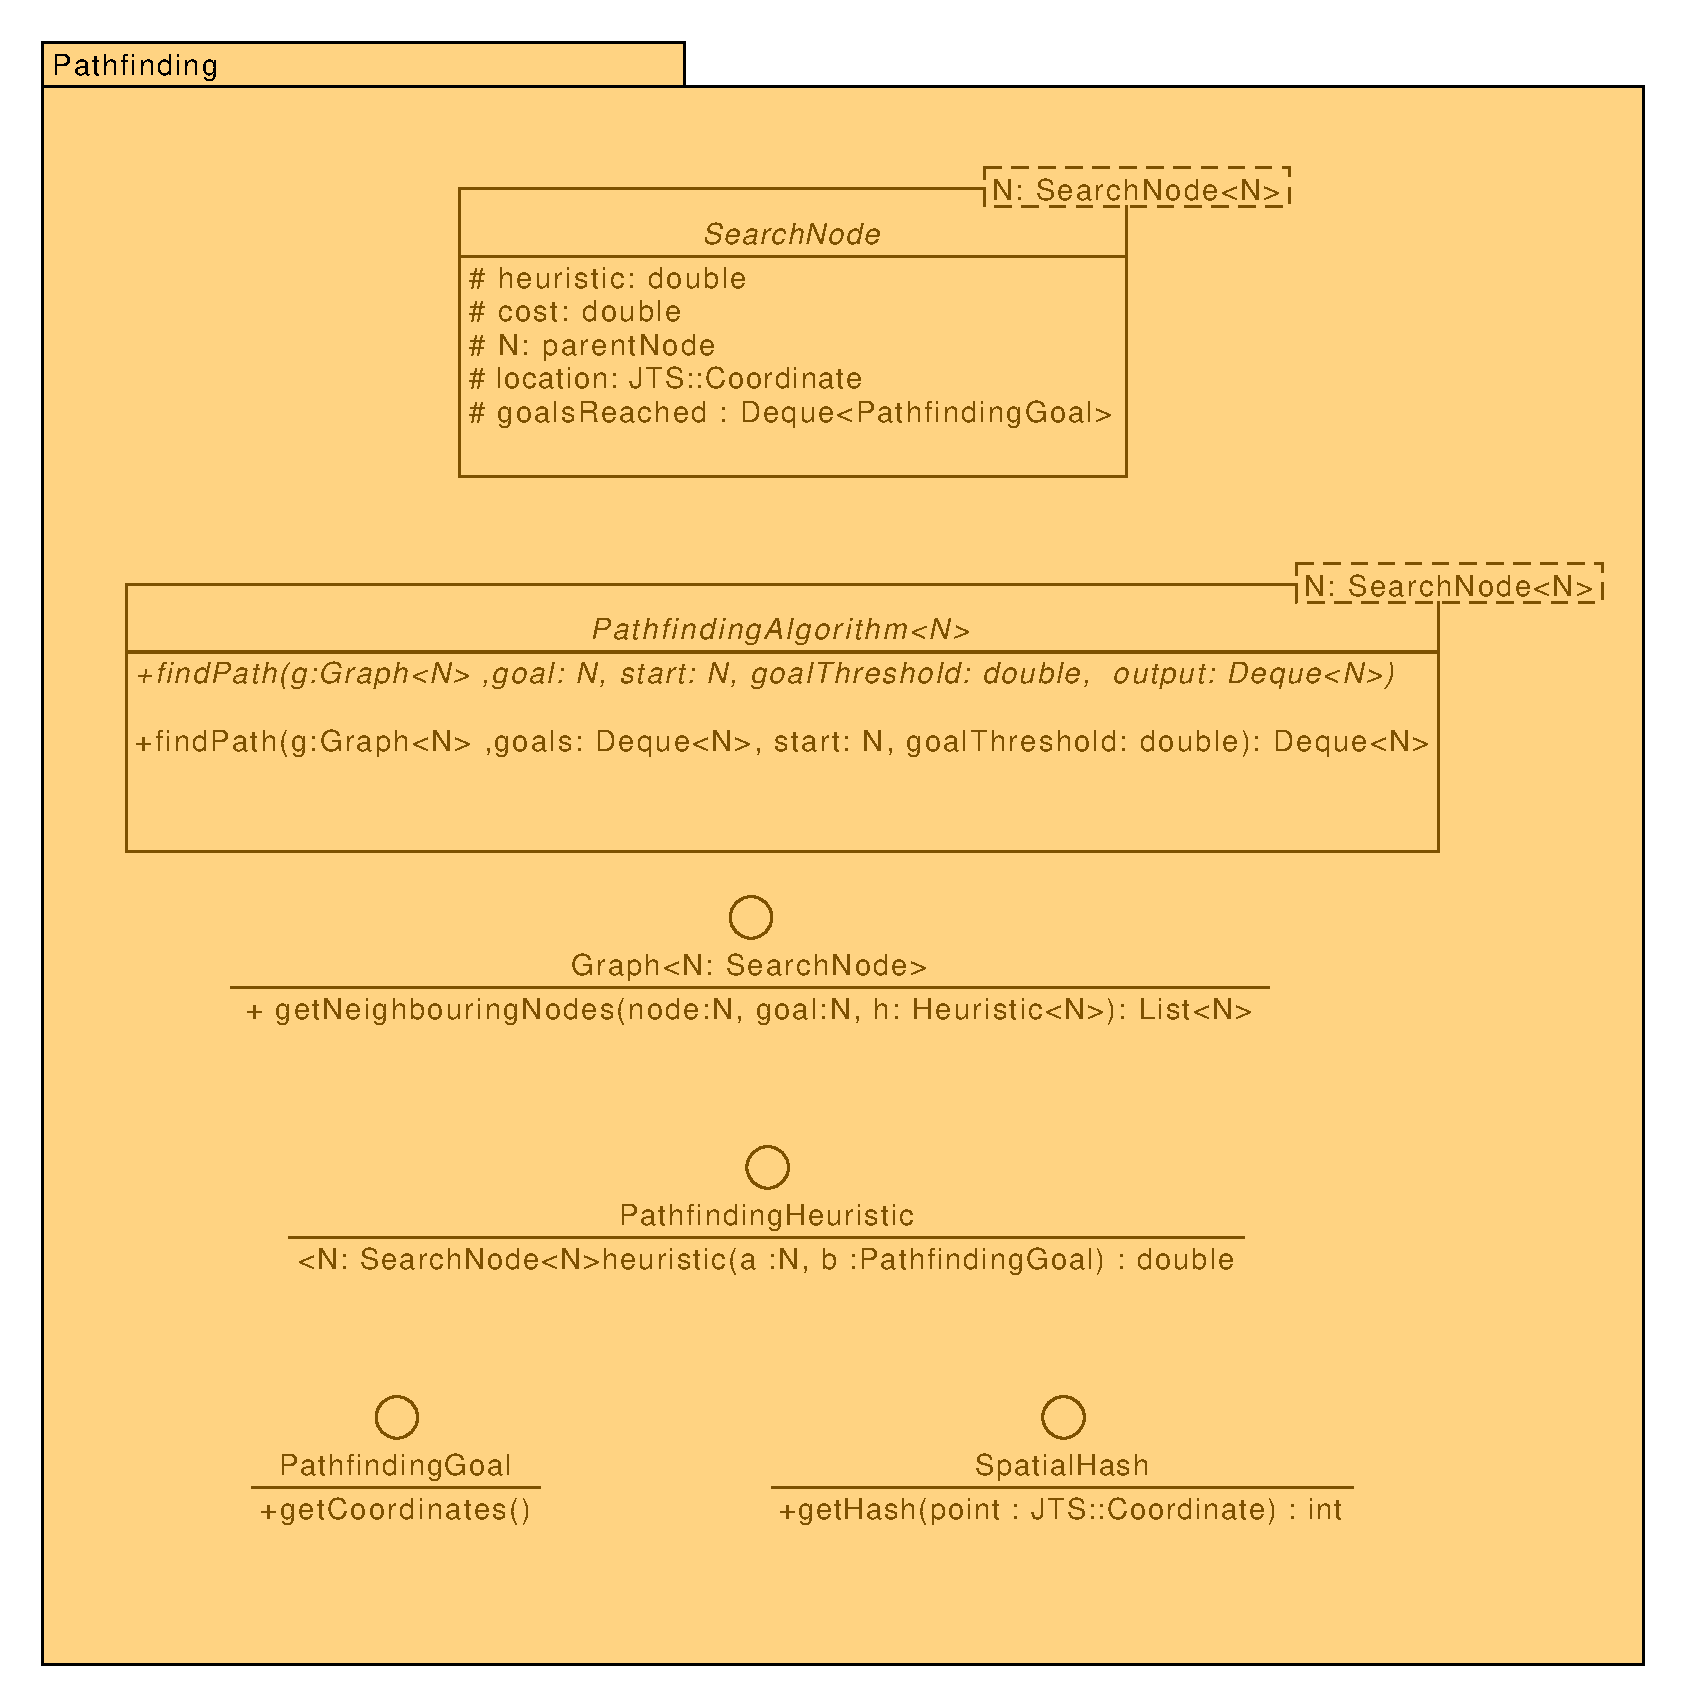
\includegraphics[width=\columnwidth]{diagrams/pathfinding.uxf.pdf}
    \caption{UML diagram of the pathfinding module}
    \label{fig:pathfinding}
\end{figure}
\begin{figure}[H]
    \centering
    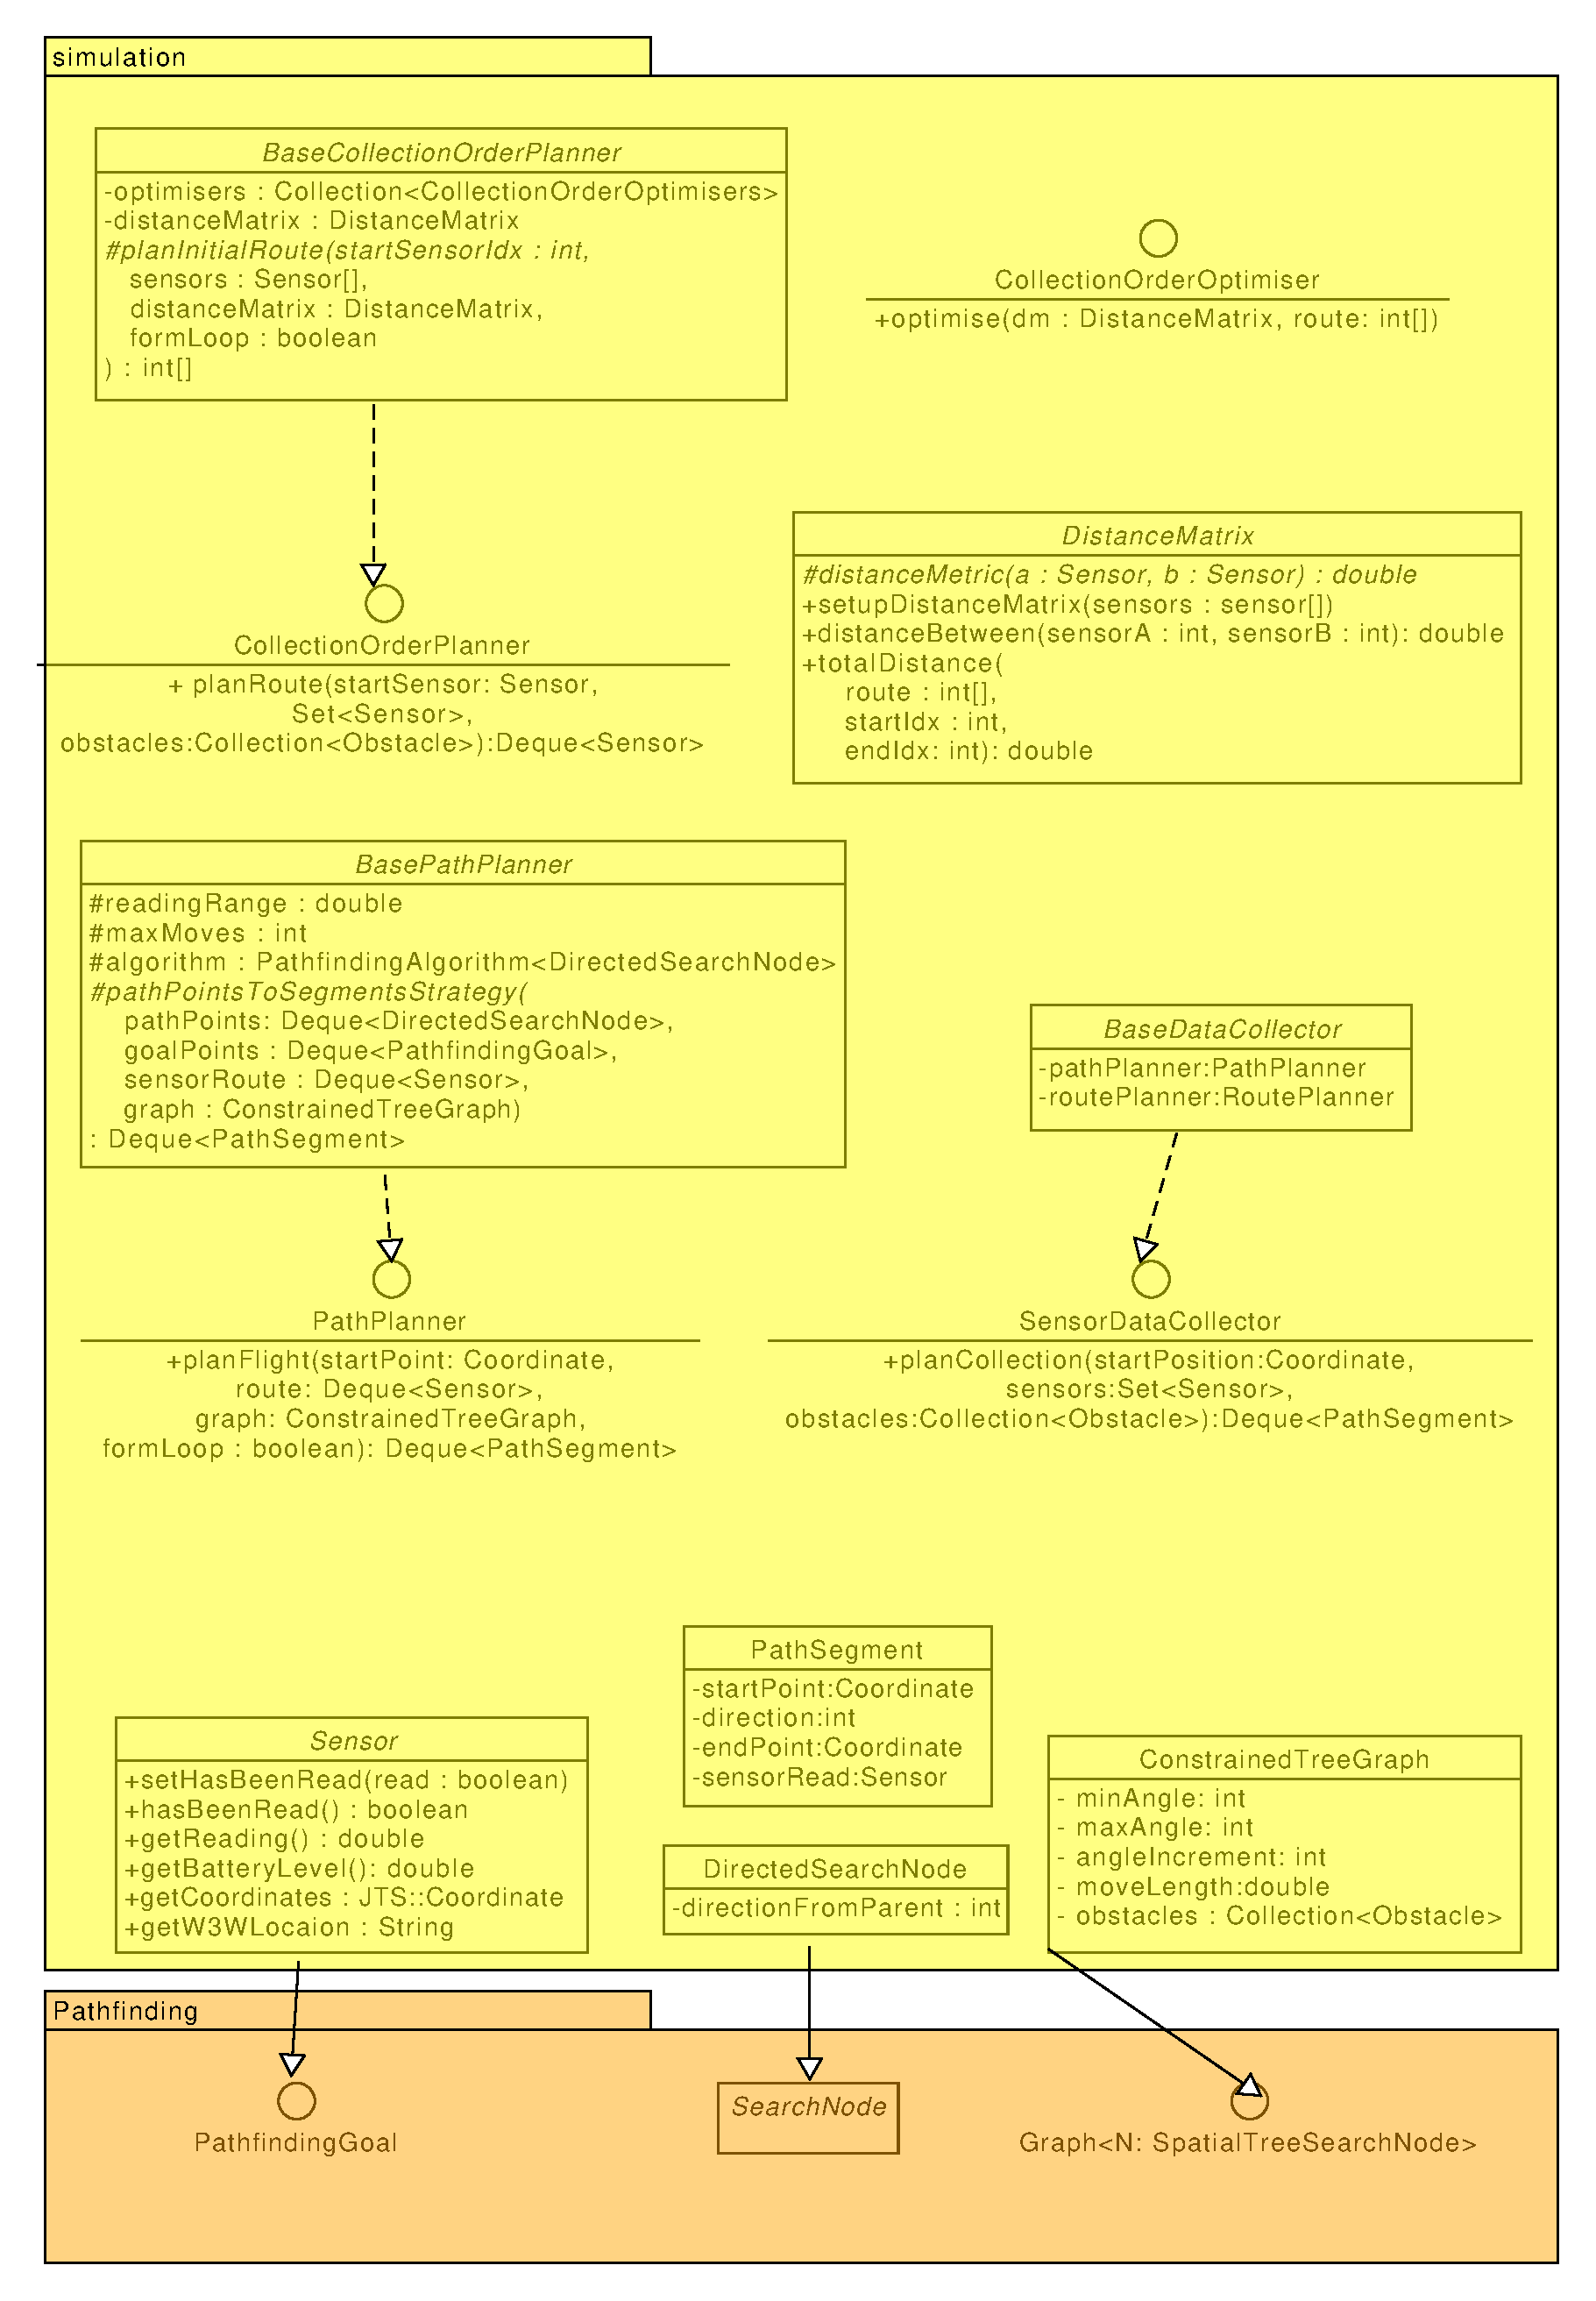
\includegraphics[width=\columnwidth]{diagrams/simulation.uxf.pdf}
    \caption{UML diagram of the Simulation module}
    \label{fig:simulation}
\end{figure}
\section{Class Documentation}
\section{Drone Control Algorithm}
\subsection{TSP Solver}

\lstdefinestyle{mystyle}{
    % backgroundcolor=\color{backcolour},
    % commentstyle=\color{codegreen},
    % keywordstyle=\color{magenta},
    % numberstyle=\tiny\color{codegray},
    % stringstyle=\color{codepurple},
    % basicstyle=\ttfamily\footnotesize,
    % breakatwhitespace=false,
    % breaklines=true,
    % captionpos=b,
    % keepspaces=true,
    % numbers=left,
    % numbersep=5pt,
    % showspaces=false,
    % showstringspaces=false,
    % showtabs=false,
    % tabsize=2,
    % numberfirstline=false,
    mathescape,
    literate=
        {=}{$\leftarrow{}$}{1}
        {==}{$={}$}{1}
        {!=}{$\neq$}{1}
        {leq}{$\leq{}$}{1}
        {nullset}{$\emptyset$}{1}
        {geq}{$\geq{}$}{1},
    morekeywords={Let,While,ArgMax,ArgMin, Function, For, If, return, Return, Algorithm, Skip},
}

\begin{figure}[H]
    \begin{lstlisting}[style=mystyle]
        Algorithm NearestInsertion:
            Let R be the sensor nearest to the starting point
            Let U = unvisited sensors
            Let T = [R] be the current tour (implicitly looping)

            While U != nullset:
                R = $\argmin_{s\in R}$ distanceToTour(s) 
                i = $\argmin_{i\in I(T)}$ insertionCost(i,R)
                T = T with R inserted at i
                U = U - {R}
            
            Return T

        Function distanceToTour(s):
            minimum = $\infty$
            For t in T:
                If dist(s,t) < minimum:
                    minimum = dist(s,t)
            Return minimum
        
        Function insertionCost(i,s):
            N = T with s inserted at i
            Return euclidian length of N
        

    \end{lstlisting}
    \caption{Nearest Insertion TSP solver}
    \label{alg:ni}
\end{figure}

The more general part of the problem is selecting the collection order of the sensors on any given day.
Assuming the drone already has the data for the appropriate collection day, it must decide on a visiting order of the sensors.
\par 
For this part many techniques were tried, and experimentation proved that applying the Nearest Insertion heuristic together with a euclidian distance matrix was an adequate solution. 
At each step we chose the sensor which is closest to one of the sensors present in the tour already - the first sensor is the one nearest to the starting point -, and insert it in a way which minimises the cost.
If U is the set of unvisited sensors and T is set of sensors in the tour, at each step we pick the sensor s such that:
\begin{equation}
    \exists s,\exists k \in T,\forall o\in U.distance(s,k) < distance(o,k)
\end{equation} 
and insert it into the tour between consecutive sensors $i,j \in T$ such that the cost of the tour is minimized.
\\
Following this initial pass, 2-opt optimisations are applied to the route to remove crossings in the graph and further reduce the cost.
The 2-opt algorithm in each pass checks if reversing any sub-segment of all possible sub-segments of a full tour reduces it's cost, and if so keeps the reversal. 
The passes are repetead until improvements fall under a threshold of 0.00003 degrees

This alrogithm turns out to be pareto-optimal \cite{metric-tsp} among a family of cutting-edge algorithms for problem sizes of between 30-50 vertices.
Pareto-optimality means that this algorithm was either finding the best path compared to the other algorithms, or was finding one the quickest. It also happens that 
this algorithm is just a variation of Prim's algorithm as in this process we find the minimum spanning tree of the implicit graph, therefore Nearest insertion is actually a 
2-approximation algorithm \cite{2-approximation-ni} of the optimal solution.
\subsection{Generating neighbour nodes}
All the other sections of the algorithm make use of the "neighbour" function, i.e. the function which generates neighbour nodes for any node representing 
a point on the map.

This is done using the Bounding Volume Hierarchy data structure. The structure allows for logarithmic time lookups of possibly colliding obstacles (with any shape).
We do this by creating a binary tree whose nodes are defined by an Axis Aligned Bounding Volume enveloping all the obstacles present in the leaf nodes underneath the node.
The root node then envelops all the obstacles present in the hierarchy.
\par
When creating the tree we find the axis along which the difference between the extremal coordinates of the AABB's is the largest, i.e. the "longest axis".
We then pick a splitting point on the axis and partition the shapes into the left and right sub trees according to which side of the splitting point they're on.
\par 
With this setup, the structure can tell us which obstacles are possibly colliding with any given shape by checking for collisions (cheaply) with the AABB's and only returning those leafs whose AABB's were collided with (possibly from both subtrees).

\subsection{Pathfinding}
\begin{figure}[H]
    \begin{lstlisting}[style=mystyle]
        Algorithm A*:
            Let R = starting node
            let G = goal coordinates
            Let O = {R} // open set
            Let V = {} // approximately visited
            
            While O != nullset:
                R = $\argmin_{o\in O}$ Fvalue(o)
                O = O - R

                If isNearGoal(R):
                    R.goalsReached = R.goalsReached + G
                    Return reconstructPath(R) // using parent references

                // generate neighbour nodes with appropriate costs and parent set to R
                // nodes colliding with obstacles or outside of boundary are excluded
                // this is done via Bounding Volume Hierarchies
                N = neighbours(R) 

                For n in N:
                    
                    hash = cantorHash(n.x,n.y)

                    If hash in V:
                        Skip n
                    
                    V = V + hash
                    O = O + n
            
            // no path found
            Return []

        Function Fvalue(n):
            Return dist(n,G)*1.5 + cost(n)

        Function cantorHash(x,y):
            Let gridWidth = $\frac{1}{75} * 0.0003 $
            Let gridX,gridY = coordinates of center of drone confinement area 
            nx,ny = (x - gridX)/gridWidth,(y - gridY)/gridWidth
            nx,ny = makePositive($\lfloor nx \rfloor$),makePositive($\lfloor ny \rfloor$)

            return $\lfloor$(((0.5 * (nx + ny)) * (nx + ny + 1)) + ny)$\rfloor$;
        
        Function makePositive(n):
            If n $\geq$ 0:
                Return $2n$
            Otherwise:
                Return $-2n - 1$
               
            
            
    \end{lstlisting}
    \caption{Custom A* pathfinding algorithm}
    \label{alg:a*}
\end{figure}

Pathfinding between any two points on the plane was carried out using the A* tree search algorithm with the euclidian distance heuristic. 
The algorithm is just a modified breadth-first search, where the search nodes are picked in order of least f value which is defined as:
\begin{equation}
    f(n) = h(n) + c(n)
\end{equation}
with $c(n)$ is the cost of reaching the node n from the start state, and $h(n)$ is the approximation of the cost of reaching the goal state from the node n.
Assuming that the node in the search frontier with the smallest f value is always expanded and that the heuristic is admissible A* will return the optimal path.

A naive application of A* could not work however due to floating-point error causing the expansion of a lot of poor nodes and the sheer amount of nodes present in the frontier at any time. 
The straight-line-distance heuristic was relaxed and the new definition was the following:
\begin{equation}
    h(n) = distance(n,g) * 1.5
\end{equation}
This makes nodes closer to the goal receive much smaller heuristic values and so more direct paths to the goal are expanded first. 
This means that the returned paths are no longer optimal as the heuristic is no longer admissible, but since most paths would not be obstucted by buildings - this
change does not actually impact the length of the paths all that much.

Another change was the addition of a spatial hash to try and prune nodes which were approximately visited, by finding out 
their coordinates relative to a grid centered around the center of the boundary (with integer width square size), and hashing those coordinates
using a modified cantor pairing allowing for negative values

\subsection{Path segmenting}
Once we have a path of individual points, we need to convert it to a path of path segments with information about which sensor is read at each segment.
We can do this by "sliding" a window over the points and always looking at two points at a time in order. 
We call the points at each position of the windo P and N, where P is the point before N. 
The pathfinding algorithm also attaches a deque of sensors reached by each P/N.  
Multiple conversion problems arise when naively pairing up the points to create segments:

\begin{itemize}
    \item P or N may reach multiple sensors which is invalid, each P-N segment must only allow for one reading
    \item The list of points might be empty if no path is found
    \item P might reach a sensor which is illegal, only N's in each segment are allowed to read sensors (since an N point always occurs at the end of a move)
\end{itemize}

\noindent The empty list of points can be prevented by simply returning no path segments, 
the rest of the problems can be defeated if we apply a number of rules in order (portrayed in Figure \ref{fig:segmenting}):
\begin{itemize}
    \item While P attains a goal, create a proxy segment to any neighbouring node, and one back, assign the first sensor attained by P 
        to the newest back-facing segment's N node
    \item If N attains no goals, see if the next segment's P node attains any sensors, if so "steal" one away from it
    \item while N attains more than one sensor reduce the number of attained sensors by creating proxy segments as above for each
    \item If N only attains one sensor or none, create P-N path segment as normal
\end{itemize}

\begin{figure}[H]
    \centering
    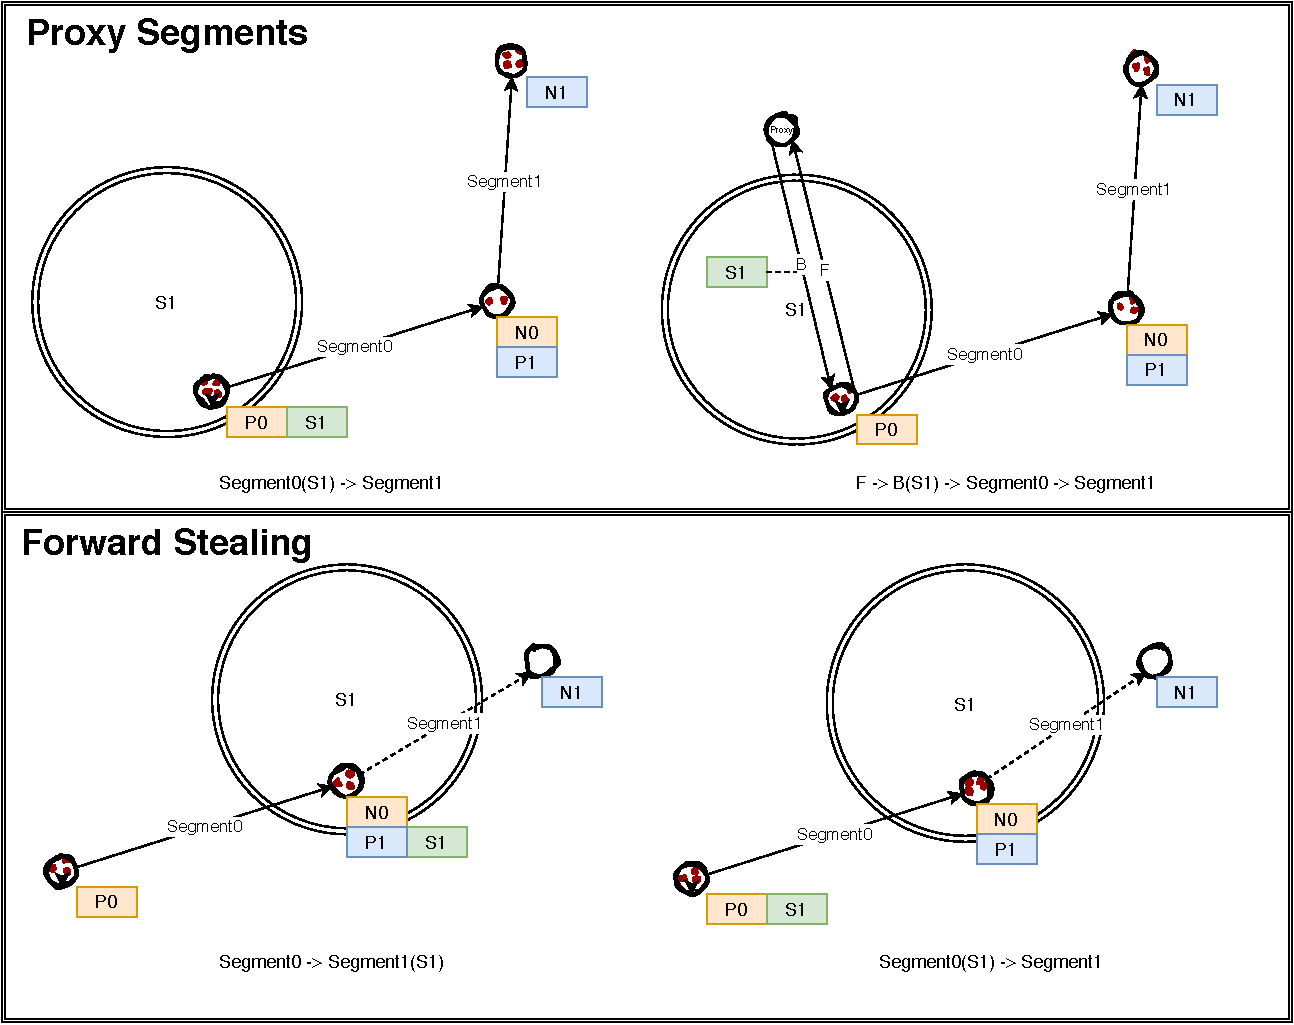
\includegraphics[width=0.7\columnwidth]{diagrams/diagram.pdf}
    \caption{Segmenting behaviours}
    \label{fig:segmenting}
\end{figure}

\subsection{Examples}
The algorithm was tested on over 35000 configurations over the data provided. 
The hardest and easiest collection days' geojson visualisations are shown below (with the algorithm set to optimal parameters as given above) 
\begin{figure}[H]
    \centering
    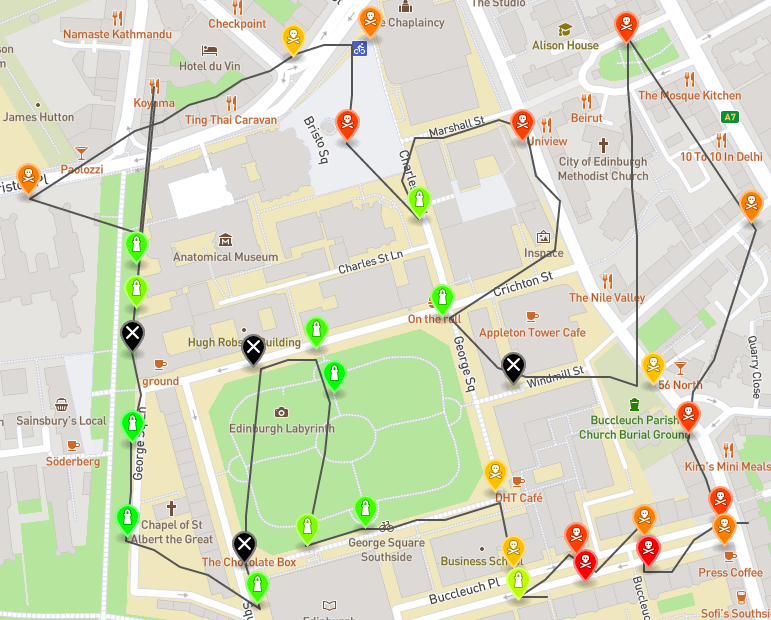
\includegraphics[width=0.6\columnwidth]{diagrams/hard-day.png}
    \caption{geojson.io rendering of hardest collection at day 9-2-2020 with a starting point of -3.19087,55.945778, with 111 moves}
    \label{fig:simulation}
\end{figure}
\begin{figure}[H]
    \centering
    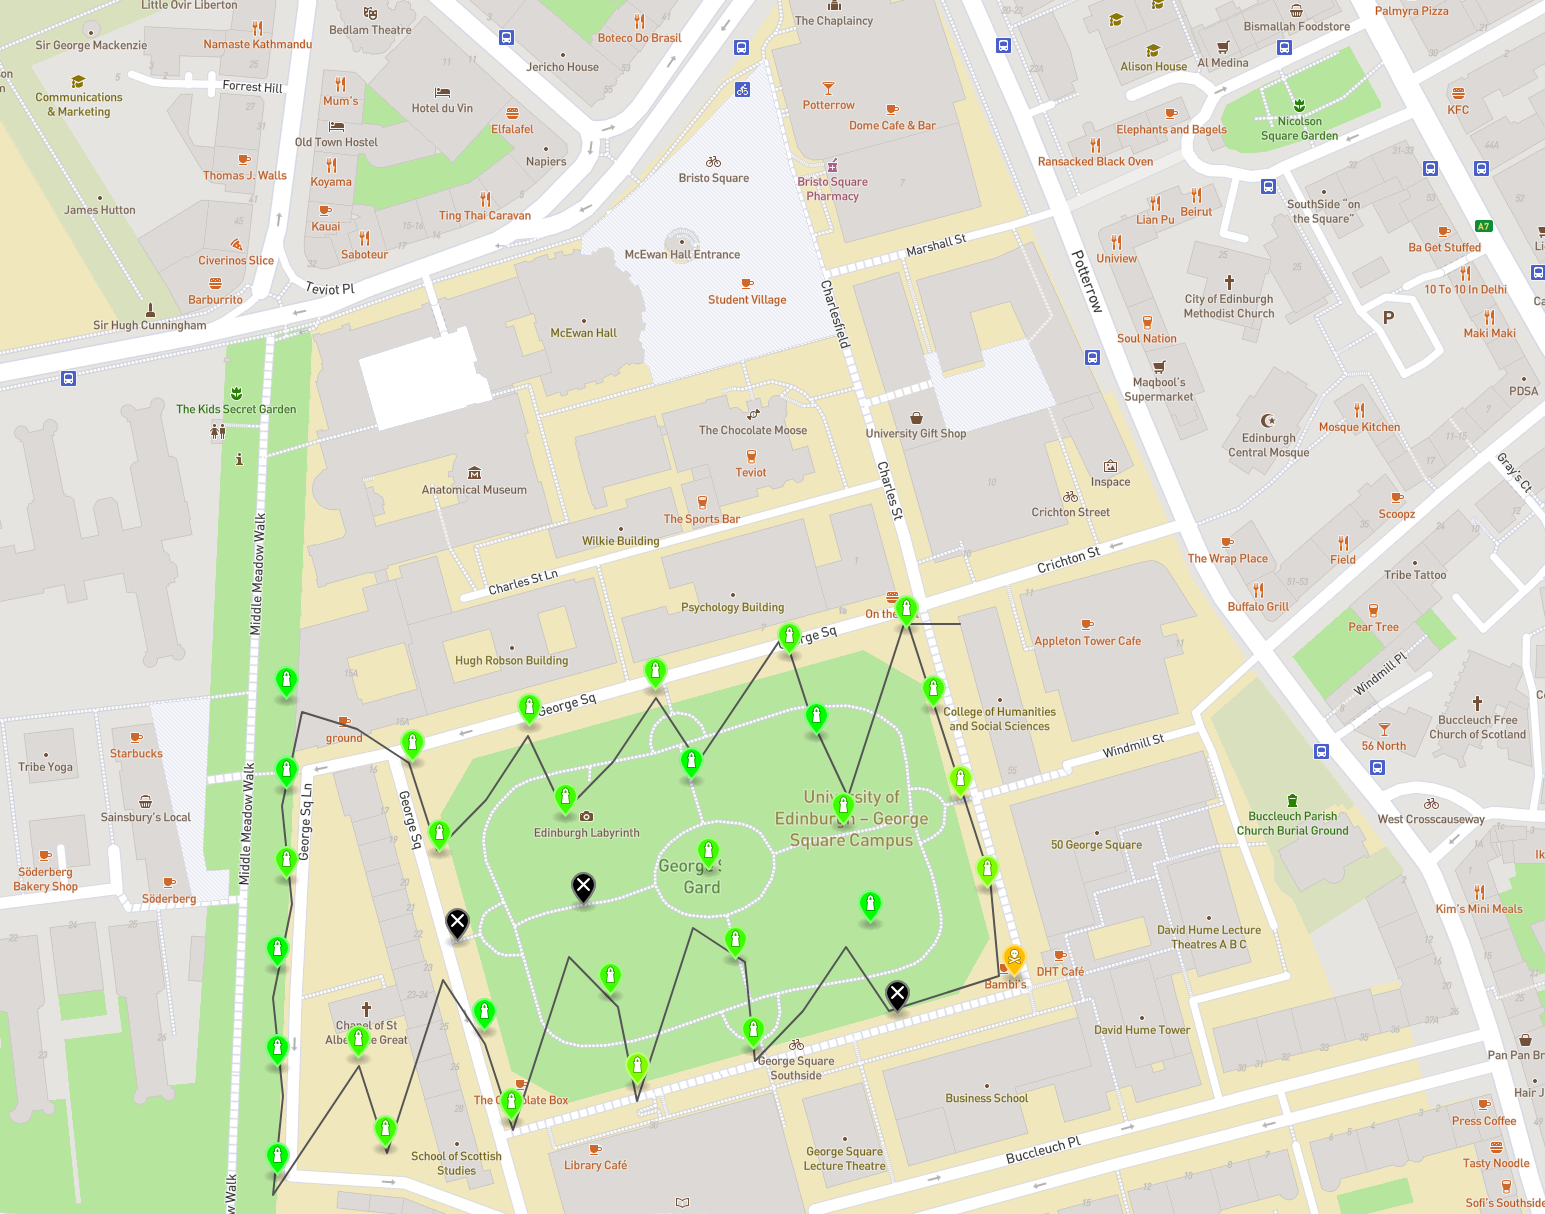
\includegraphics[width=0.6\columnwidth]{diagrams/easy-day.png}
    \caption{geojson.io rendering of easiest collection at day 2-1-2021 with a starting point of -3.1878,55.9444, with 46 moves}
    \label{fig:simulation}
\end{figure}

The artifacts of path segmenting are evident in the harder day, where the drone wanders near closely spaced sensors on the bottom right it creates a horizontal 
proxy segment. But overall the algorithm manages very well, never carrying out the collection in more than 111 moves and averaging at 90 moves $\pm$ 6.7. Execution times averaged at 103ms.
\begin{thebibliography}{9}

\bibitem{metric-tsp} 
The Metric Travelling Salesman Problem:
The Experiment on Pareto-optimal
Algorithms,
Sergey Avdoshin, E.N.Beresneva
2017.
\bibitem{2-approximation-ni} 
https://aswani.ieor.berkeley.edu/teaching/FA13/151/lecture\_notes/ieor151\_lec17.pdf,
The Traveling Salesman Problem
Professor Z. Max Shen

\end{thebibliography}

\end{document}